% USE PDFLatex!
% to correctly render Swedish characters

\documentclass{popsci}

\usepackage[utf8]{inputenc}
\usepackage[swedish, english]{babel}

\usepackage{fancyhdr}
\usepackage{titling}
\usepackage{color}
\usepackage{colortbl}
\usepackage{graphicx}
\usepackage{flushend}
\usepackage{lmodern}


% Please specify the presentation date
\presentationsdag{2022-06-07}

% use either of these commands to specify the title of your thesis
\examensarbete{Drones for Sea Rescue: Lab and Field Experiments on Camera Gimbal Control}
% To create a title in two rows, leave examensarbete blank and fill in examensarbeteTwoRows.
%\examensarbeteTwoRows{}{}
\student{Alexander Sandström}
%\students{Magnus Hultin}{Mr X}
\supervisor{William Tärneberg (LTH), Fredrik Falkman (Sjöräddningssällskapet)}
\examiner{Maria Kihl(LTH)}

% Your pop-sci title should be different (more catchy) than your thesis title
\title{Drönare som understöd vid sjöräddning}


\begin{document}

% not more than 4 rows!
%\theabstract{Applikations-specifika processorer är allt mer vanligt för få ut rätt prestanda med så lite resurser som möjligt. Detta arbete har en parametrisk modell för att kunna testa hur mycket resurser som behövs för en specifik applikation.}
\theabstract{Sjöräddningssällskapet (SSRS) driver idag ett projekt där man utforskar möjligheten att använda drönare för att understödja räddningspersonal vid uttryckning till havs. I detta arbete har en mjukvara för att styra kameran ombord på drönaren implementerats och utvärderats i labb och under riktig flygning.}

{\noindent Vid en uttryckning till havs kan små skillnader i tid vara skillnaden mellan en lyckad räddning och en katastrof. För att kunna ge räddningspersonalen bättre beslutsunderlag i ett så tidigt skede som möjligt driver SSRS ett innovationsprojekt där man undersöker användningen av drönare för snabbt förse sjöräddarna med bilder från en olycksplats.

\begin{figure}[!bth] % Use pictures in your pop-vet!
    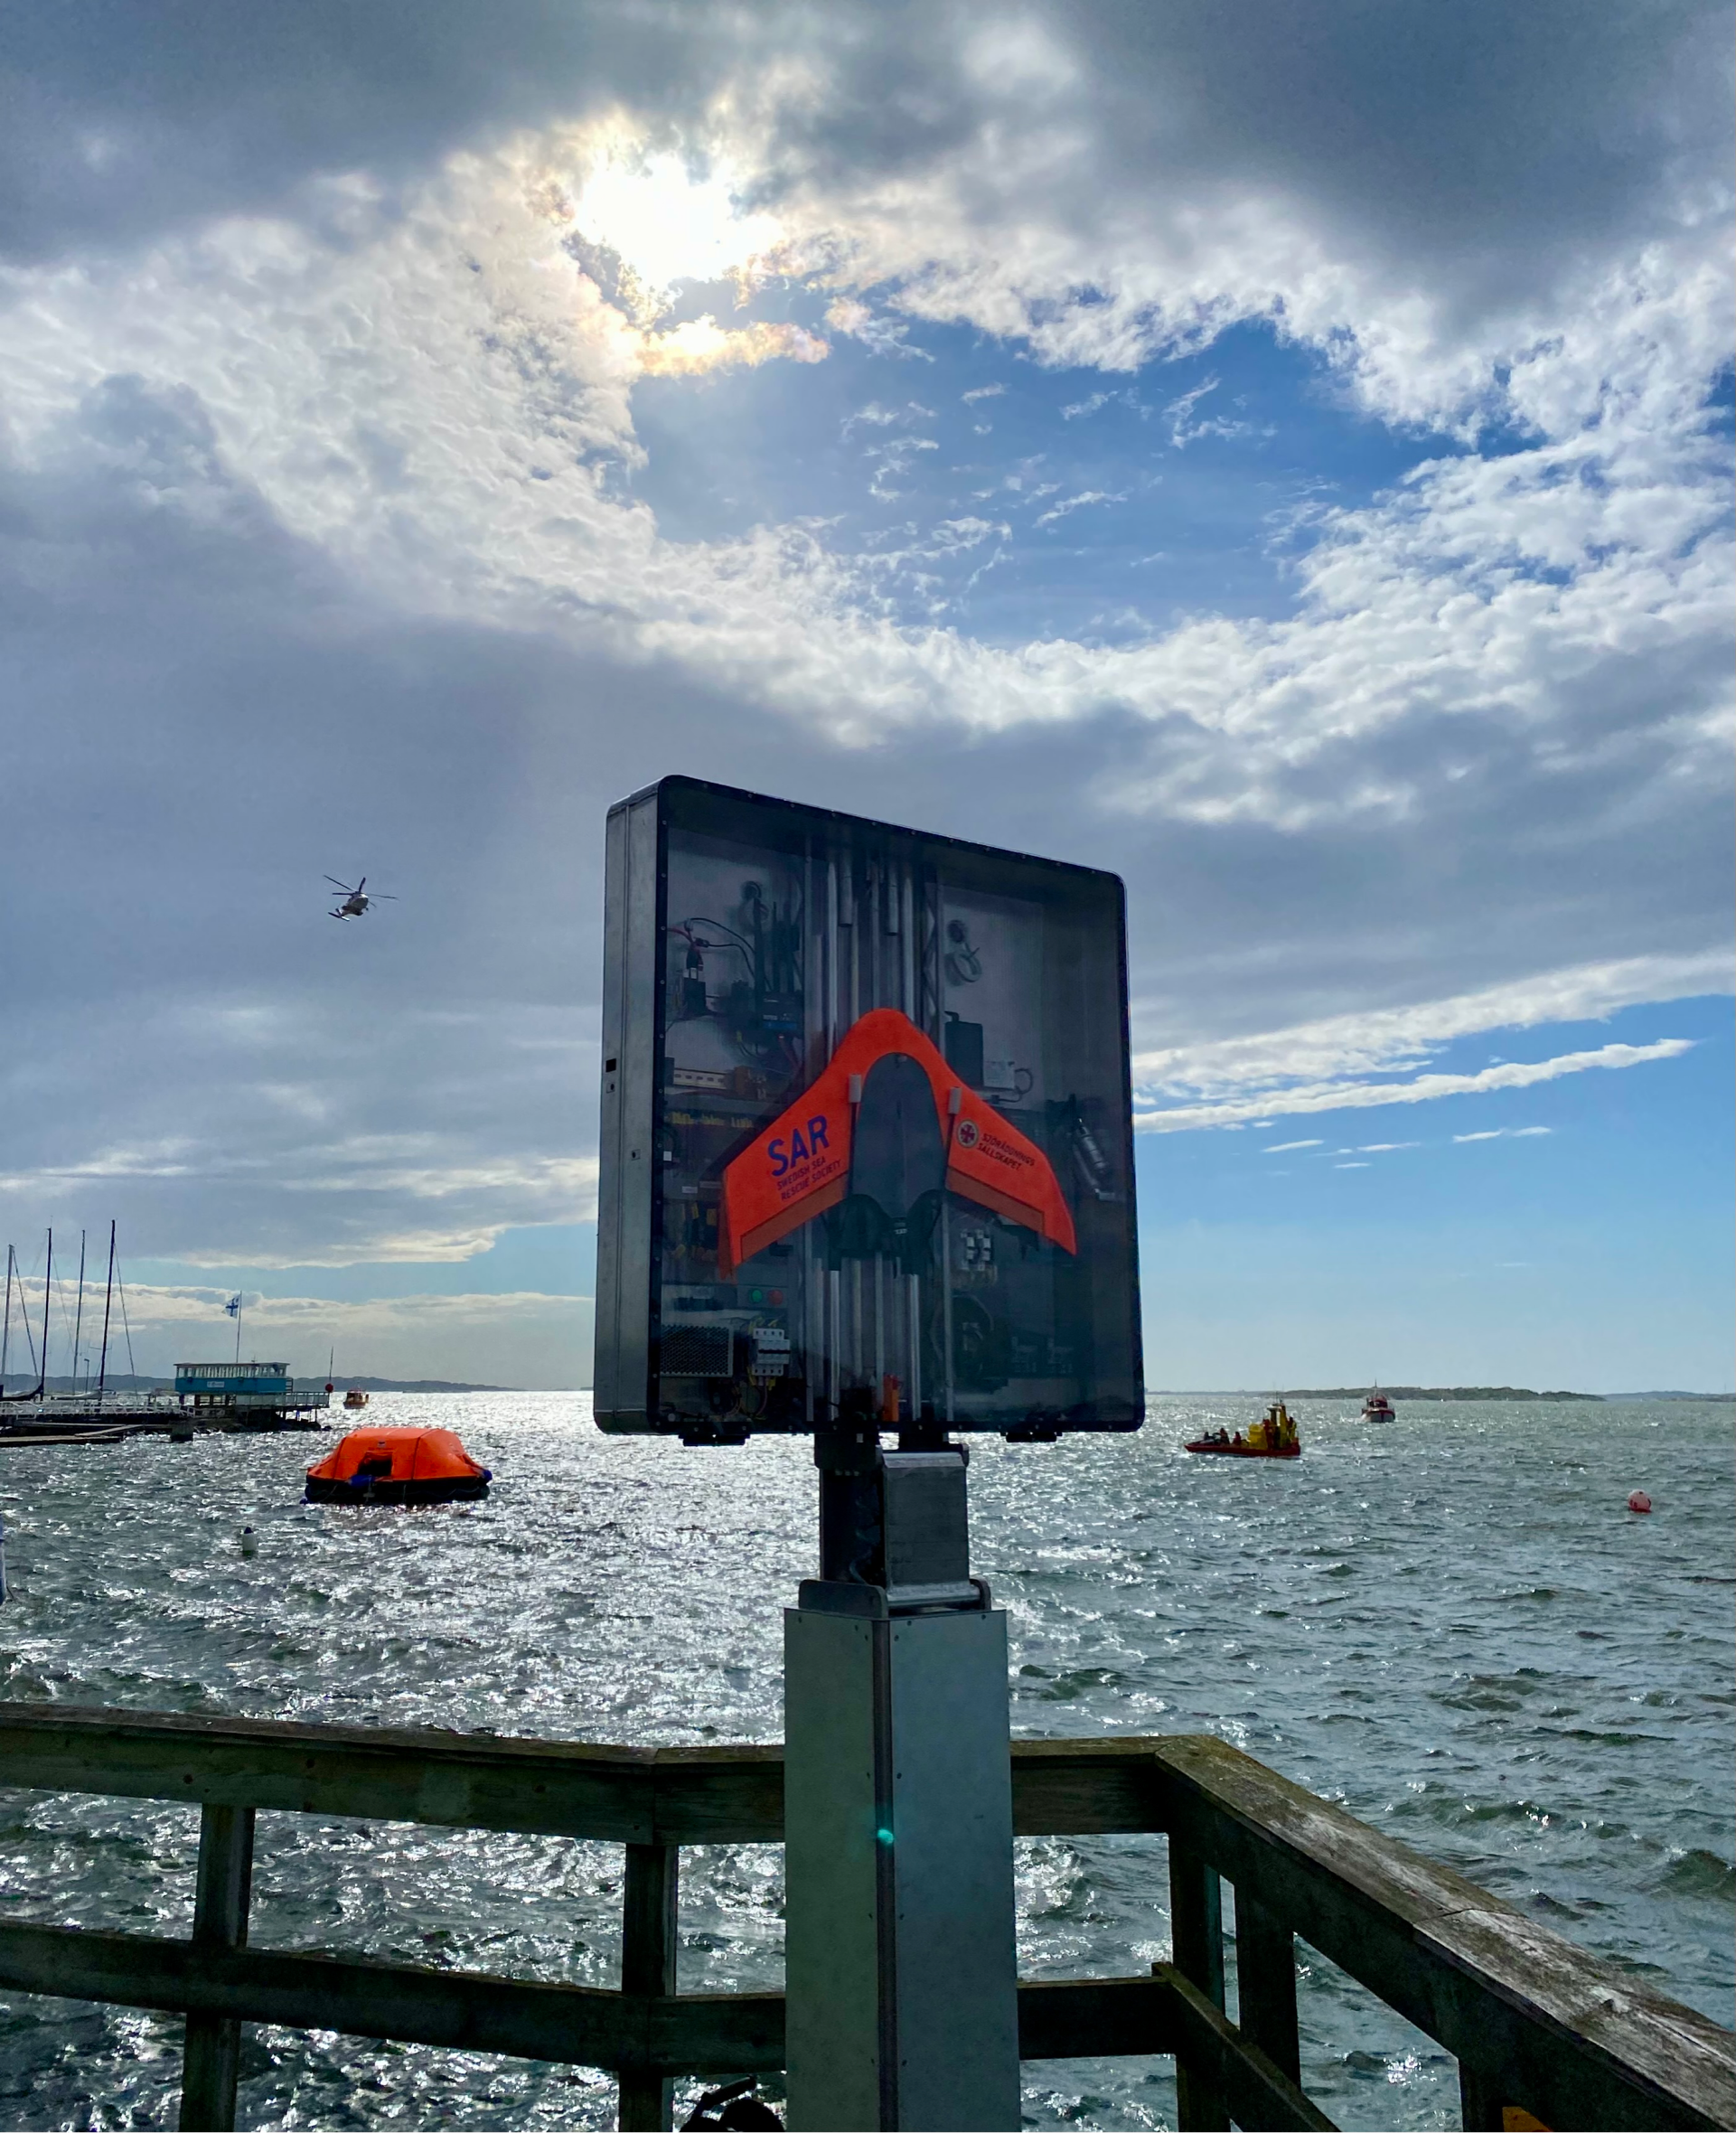
\includegraphics[trim={0 20cm 0 30cm},width=\columnwidth, clip]{../images/dronepic.png} 
    %\caption{En fin bild}
\end{figure}

Drönaren är en så kallad fastvinge, vilket gör att den både är snabbare och mer energieffektiv än den mer vanliga rotordrönaren. Det innebär att den kan vara snabbt på plats vid en olycka för att sedan ge kontinuerligt bildstöd från luften under längre tid än vad en rotordrönare klarat av. På undersidan av drönaren sitter en kamera monterad på en gimbal som gör det möjligt att vrida kameran i alla tre axlar.

Tidigare kunde SSRS bara styra kameran med hjälp av GPS-punkter som placerades ut på en karta. Detta var inte en så effektiv process då en GPS-punkts exakthet kan försämras av många olika störningar. SSRS ville därmed se vilka möjligheter som fanns att justera kameravinkeln snabbare med hjälp av exempelvis piltangenter eller en joystick.

Mitt examensarbete har gått ut på att implementera manuell gimbal-styrning och inom arbetet har jag utfört två experiment: det första ett labbexperiment där drönaren stått stilla och försökspersonen fått en uppgift att med kameran. Jag har sedan tittat på hur bra de klarar av uppgiften när en fördröjning introduceras i systemet. Det visade sig att fördröjning försämrade operatörens förmåga att klara av uppgiften, men att en likvärdig ökning i fördröjning hade större effekt vid en redan högre fördröjning.

Det andra experimentet gjordes under en riktig flygning i Göteborgs skärgård där jag kollade på när manuell styrning var att föredra över det tidigare nämnda GPS-läget. I och med stora fördröjningar i det mobila nätverket lämpade sig manuell kamerastyrning bäst när drönaren flög rakt och man ville titta omkring sig. Det gick även bra att följa ett objekt. 
}
\end{document}
